\let\negmedspace\undefined
\let\negthickspace\undefined
\documentclass[journal]{IEEEtran}
\usepackage[a5paper, margin=10mm, onecolumn]{geometry}
%\usepackage{lmodern} % Ensure lmodern is loaded for pdflatex
\usepackage{tfrupee} % Include tfrupee package

\setlength{\headheight}{1cm} % Set the height of the header box
\setlength{\headsep}{0mm}     % Set the distance between the header box and the top of the text

\usepackage{gvv-book}
\usepackage{gvv}
\usepackage{algorithmicx} % Ensure algorithmicx is loaded explicitly
\usepackage{cite}
\usepackage{amsmath,amssymb,amsfonts,amsthm}
\usepackage{graphicx}
\usepackage{textcomp}
\usepackage{xcolor}
\usepackage{txfonts}
\usepackage{listings}
\usepackage{enumitem}
\usepackage{mathtools}
\usepackage{gensymb}
\usepackage{comment}
\usepackage[breaklinks=true]{hyperref}
\usepackage{tkz-euclide} 
\usepackage{listings}
% \usepackage{gvv}                                        
\def\inputGnumericTable{}                                 
\usepackage[latin1]{inputenc}                                
\usepackage{color}                                            
\usepackage{array}                                            
\usepackage{longtable}                                       
\usepackage{calc}                                             
\usepackage{multirow}                                         
\usepackage{hhline}                                           
\usepackage{ifthen}                                           
\usepackage{lscape}
\usepackage{algorithm}
\usepackage{algpseudocode}

\renewcommand{\thefigure}{\theenumi}
\renewcommand{\thetable}{\theenumi}
\setlength{\intextsep}{10pt} % Space between text and floats


\numberwithin{equation}{enumi}
\numberwithin{figure}{enumi}
\renewcommand{\thetable}{\theenumi}

% Marks the beginning of the document
\begin{document}
\bibliographystyle{IEEEtran}

\title{Digital Clock}
\author{EE24BTECH11049 \\ Patnam Shariq Faraz Muhammed}


% \maketitle
% \newpage
% \bigskip
{\let\newpage\relax\maketitle}
\begin{abstract}
    This report focuses on implementation of a digital clock using an AVR microcontroller, displaying time on both a 7-segment display and an LCD. It allows users to manually set the time and switch between multiple time zones using buttons. The clock maintains accurate time using internal timers and does not require an external RTC module. Time zone adjustments are made using pre-defined offsets. The system is efficient, user-friendly, and suitable for embedded applications where real-time clock management is necessary. 
\end{abstract}
\newpage
\tableofcontents
\newpage
\section{Introduction}
This project is an AVR microcontroller-based digital clock that displays time using both a 7-segment display and an LCD. It allows users to set the time, change time zones, and interact using buttons. The clock uses internal timers for timekeeping and multiplexing the 7-segment display. The implementation emphasizes efficiency by using bitwise operations instead of arithmetic operations like ++ and -- in some areas in which I was able to understand properly. 

\section{Hardware Components}
The following are components required for the project
\begin{itemize}
    \item Six 7-segment displays
    \item Six resistors (220$\Omega$)
    \item Arduino UNO
    \item Breadboard
    \item Jumper wires
    \item Cell phone (to power the Arduino)
\end{itemize}

\section{Hardware Setup}
The wiring process involves connecting the 7447 decoder, segment lines, and common anodes to the Arduino pins.
\begin{figure}[H]
    \centering
    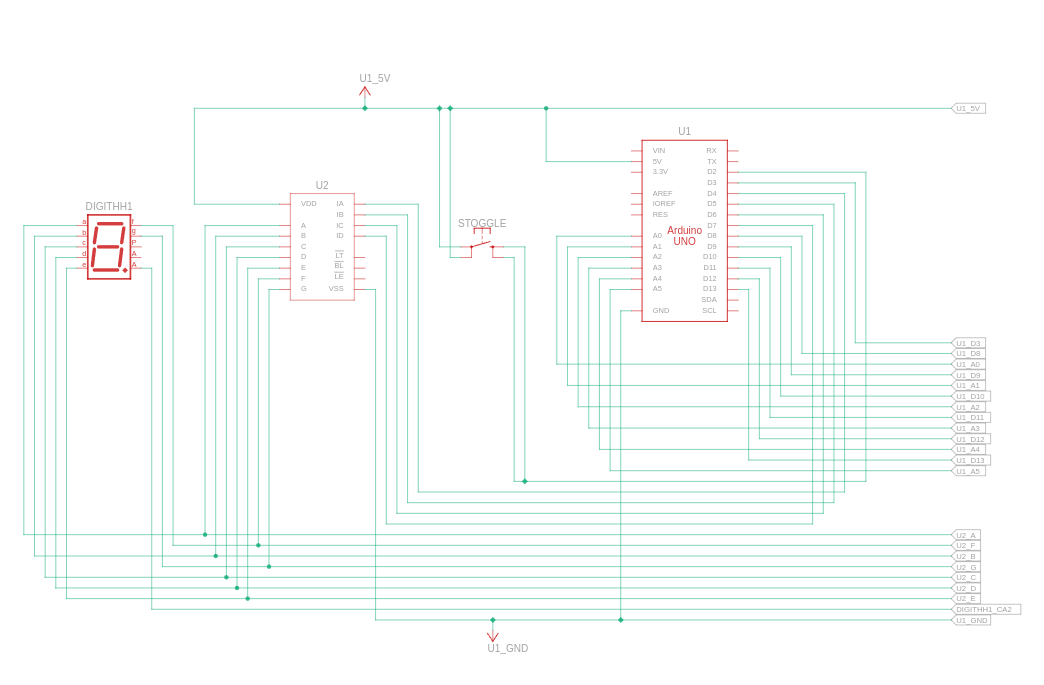
\includegraphics[width=0.9\linewidth]{figs/Pinout1.png}
    \caption{connections}
    \label{fig:enter-label}
\end{figure}
\begin{figure}
    \centering
    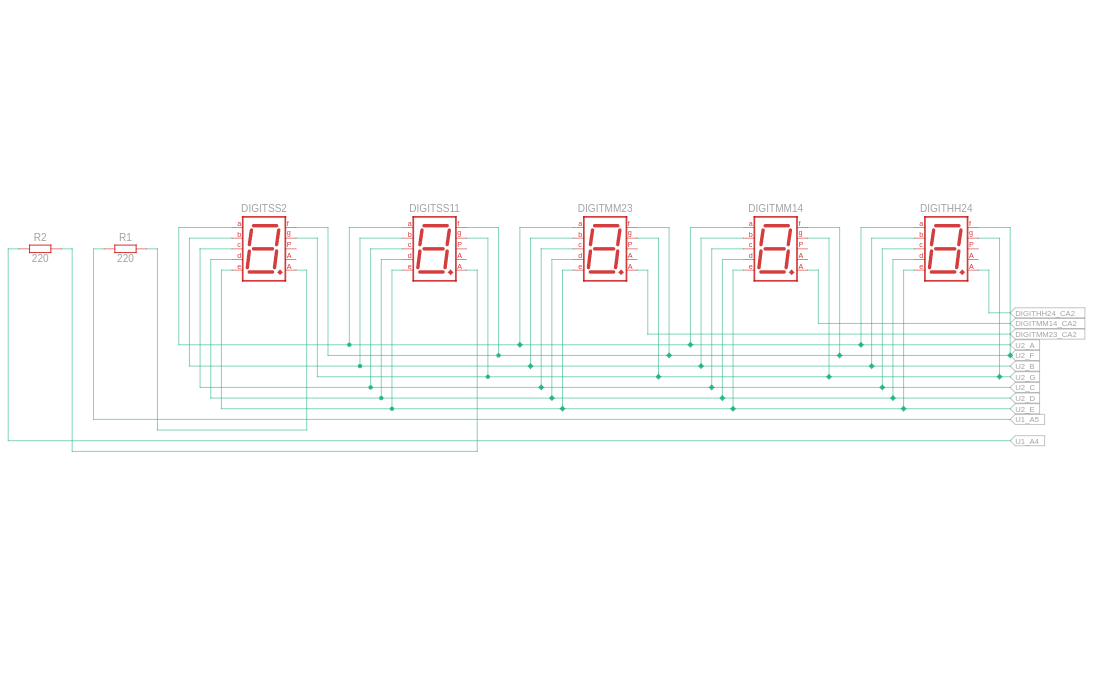
\includegraphics[width=0.9\linewidth]{figs/Pinout2.png}
    \caption{connections}
    \label{fig:enter-label}
\end{figure}
\begin{figure}
    \centering
    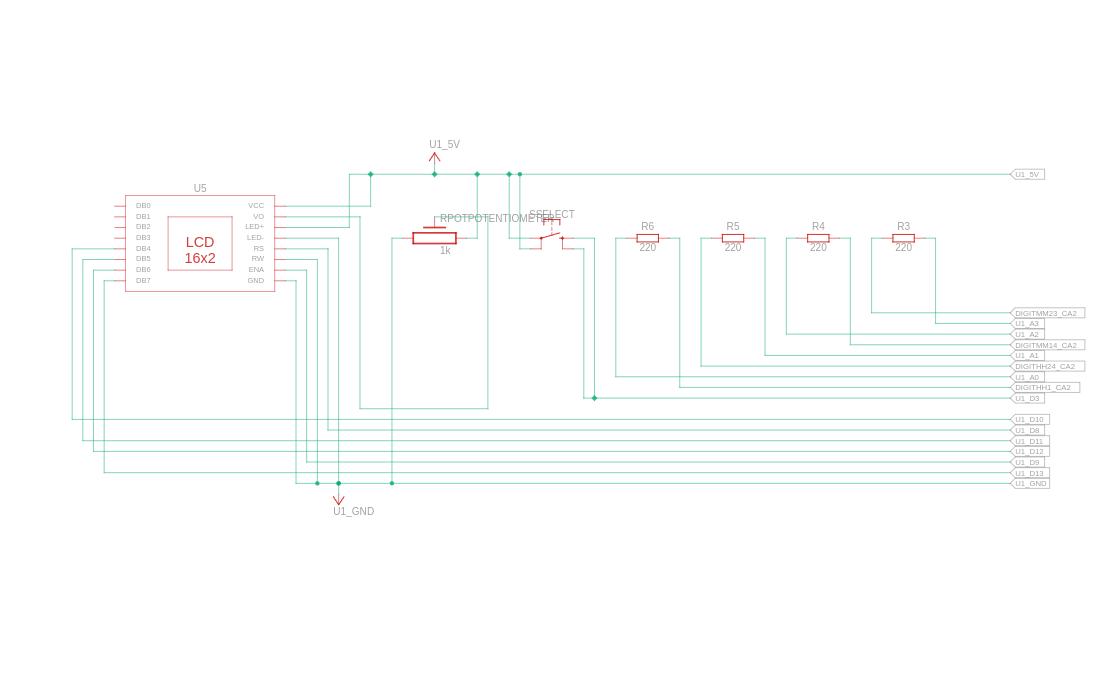
\includegraphics[width=0.9\linewidth]{figs/Pinout3.png}
    \caption{connections}
    \label{fig:enter-label}
\end{figure}
\newpage
\subsection{Connections}
\begin{enumerate}
    \item The table below shows the connections between the 7447 decoder, seven-segments, LCD and the Arduino Uno:\\

    \item Each display's common anode is connected to an Arduino analog pin through a 220$\Omega$ resistor to limit current flow.

    \item 
\end{enumerate}
\begin{table}[htbp]
\centering
\begin{tabular}{|l|l|l|}
\hline
\textbf{Component} & \textbf{Arduino Pin} & \textbf{Description} \\
\hline
\multicolumn{3}{|c|}{\textbf{LCD Display}} \\
\hline
RS & PB0 (Digital 8) & Register Select line \\
\hline
E & PB1 (Digital 9) & Enable line \\
\hline
D4 & PB2 (Digital 10) & Data line 4 \\
\hline
D5 & PB3 (Digital 11) & Data line 5 \\
\hline
D6 & PB4 (Digital 12) & Data line 6 \\
\hline
D7 & PB5 (Digital 13) & Data line 7 \\
\hline
\multicolumn{3}{|c|}{\textbf{7-Segment Display}} \\
\hline
Segment A & PD4 (Digital 4) & Segment A line \\
\hline
Segment B & PD5 (Digital 5) & Segment B line \\
\hline
Segment C & PD6 (Digital 6) & Segment C line \\
\hline
Segment D & PD7 (Digital 7) & Segment D line \\
\hline
Common HH\_1 & PC0 (Analog 0) & Hours tens digit common \\
\hline
Common HH\_2 & PC1 (Analog 1) & Hours ones digit common \\
\hline
Common MM\_1 & PC2 (Analog 2) & Minutes tens digit common \\
\hline
Common MM\_2 & PC3 (Analog 3) & Minutes ones digit common \\
\hline
Common SS\_1 & PC4 (Analog 4) & Seconds tens digit common \\
\hline
Common SS\_2 & PC5 (Analog 5) & Seconds ones digit common \\
\hline
\multicolumn{3}{|c|}{\textbf{Buttons}} \\
\hline
Toggle Button & PD2 (Digital 2) & For cycling through options \\
\hline
Select Button & PD3 (Digital 3) & For selecting options \\
\hline
\end{tabular}
\caption{Arduino to Component Connections}
\end{table}
\newpage

\section{How my code works?}
\subsection{Multiplexing (7-Segment Display)}

The code uses multiplexing to display time on a 7-segment display, reducing the number of required I/O pins. This is done by:
\begin{itemize}
    \item Assigning \texttt{PORTD} (higher 4 bits) for segment values.
    \item Using \texttt{PORTC} to control the common cathode/anode lines.
    \item Using \textbf{Timer0 Interrupt Service Routine (ISR)} to rapidly cycle through digits.
\end{itemize}


\subsubsection{Multiplexing Implementation in ISR}
\begin{verbatim}
ISR(TIMER0_COMPA_vect) {
    static uint8_t digitIndex = 0;
    uint8_t digits[6] = {hours / 10, hours % 10, minutes / 10, minutes % 10, seconds / 10, seconds % 10};
    uint8_t pins[6] = {HH_1, HH_2, MM_1, MM_2, SS_1, SS_2};

    displayDigit(pins[digitIndex], digits[digitIndex]);
    digitIndex = (digitIndex + 1) % 6;
}
\end{verbatim}

\noindent The function \texttt{displayDigit()} updates the display for one digit at a time, creating the illusion of a full display through rapid switching.

\subsection{Button Functionality}

The system has two buttons:
\begin{itemize}
    \item \textbf{Toggle Button}: Cycles through options (e.g., selecting a time zone or incrementing a digit).
    \item \textbf{Select Button}: Confirms a selection.
\end{itemize}

\subsubsection{Button Press Detection}
\begin{verbatim}
bool isButtonPressed(uint8_t pin) {
    if (!(PIND & (1 << pin))) {  // Active LOW
        _delay_ms(200);  // Debounce delay
        if (!(PIND & (1 << pin))) return true;
    }
    return false;
}
\end{verbatim}

\noindent The button press is detected using \texttt{PIND} register, and a debounce delay (explained in Section~\ref{sec:debouncing}) ensures reliable operation.

\subsection{Debouncing} \label{sec:debouncing}

To prevent false triggers from mechanical button bouncing, the code implements software debouncing:
\begin{enumerate}
    \item When a button press is detected, the code waits for 200 ms.
    \item It checks if the button is still pressed.
    \item If the button remains pressed, the function returns \texttt{true}.
\end{enumerate}

\subsection{Time Zone Functionality}

The system supports eight time zones, defined as:

\subsubsection{Time Zone Selection and Adjustment}
When the user presses the toggle button, the time zone cycles through the available options. The adjustment follows:
\begin{verbatim}
if (isButtonPressed(TOGGLE_BUTTON)) {
    selectedZone = (-~selectedZone) & 7; // Cycle through zones
    int adjHours = hours - timezoneOffsets[currentZone] + timezoneOffsets[selectedZone];

    if (adjHours < 0) adjHours += 24;  // Handle negative wrap-around
    if (adjHours >= 24) adjHours -= 24; 
    hours = adjHours;
    currentZone = selectedZone;
}
\end{verbatim}

\noindent The time zone change is applied by adjusting \texttt{hours} based on the old and new offsets, with wrap-around logic for negative and overflow cases.

\subsection{Timekeeping Using Timers}

The system uses hardware timers to keep track of time. Timer1 is configured to generate an interrupt every second, which increments the seconds counter. When the seconds reach 60, the minutes counter is incremented, and similarly, when minutes reach 60, the hours counter is updated. The hours wrap around after 24 to maintain a 24-hour format.

\begin{figure}[H]
    \centering
    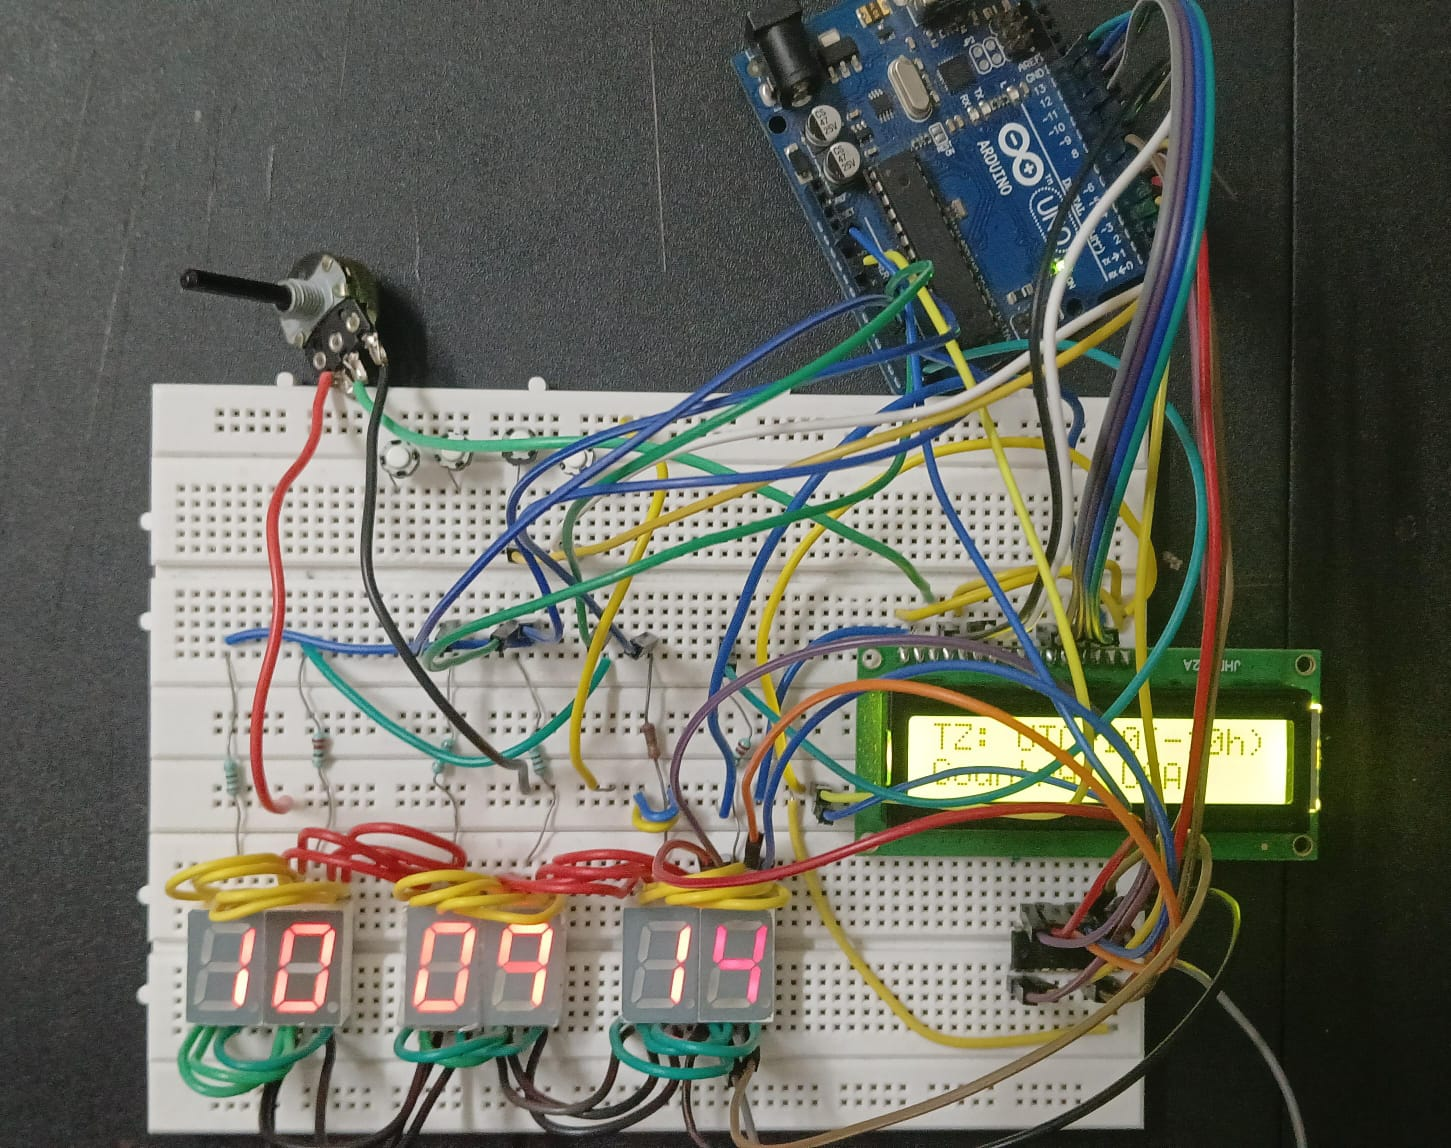
\includegraphics[width=0.8\linewidth]{figs/Clock.jpeg}
    \caption{Clock}
    \label{fig:enter-label}
\end{figure}

\begin{figure}[H]
    \centering
    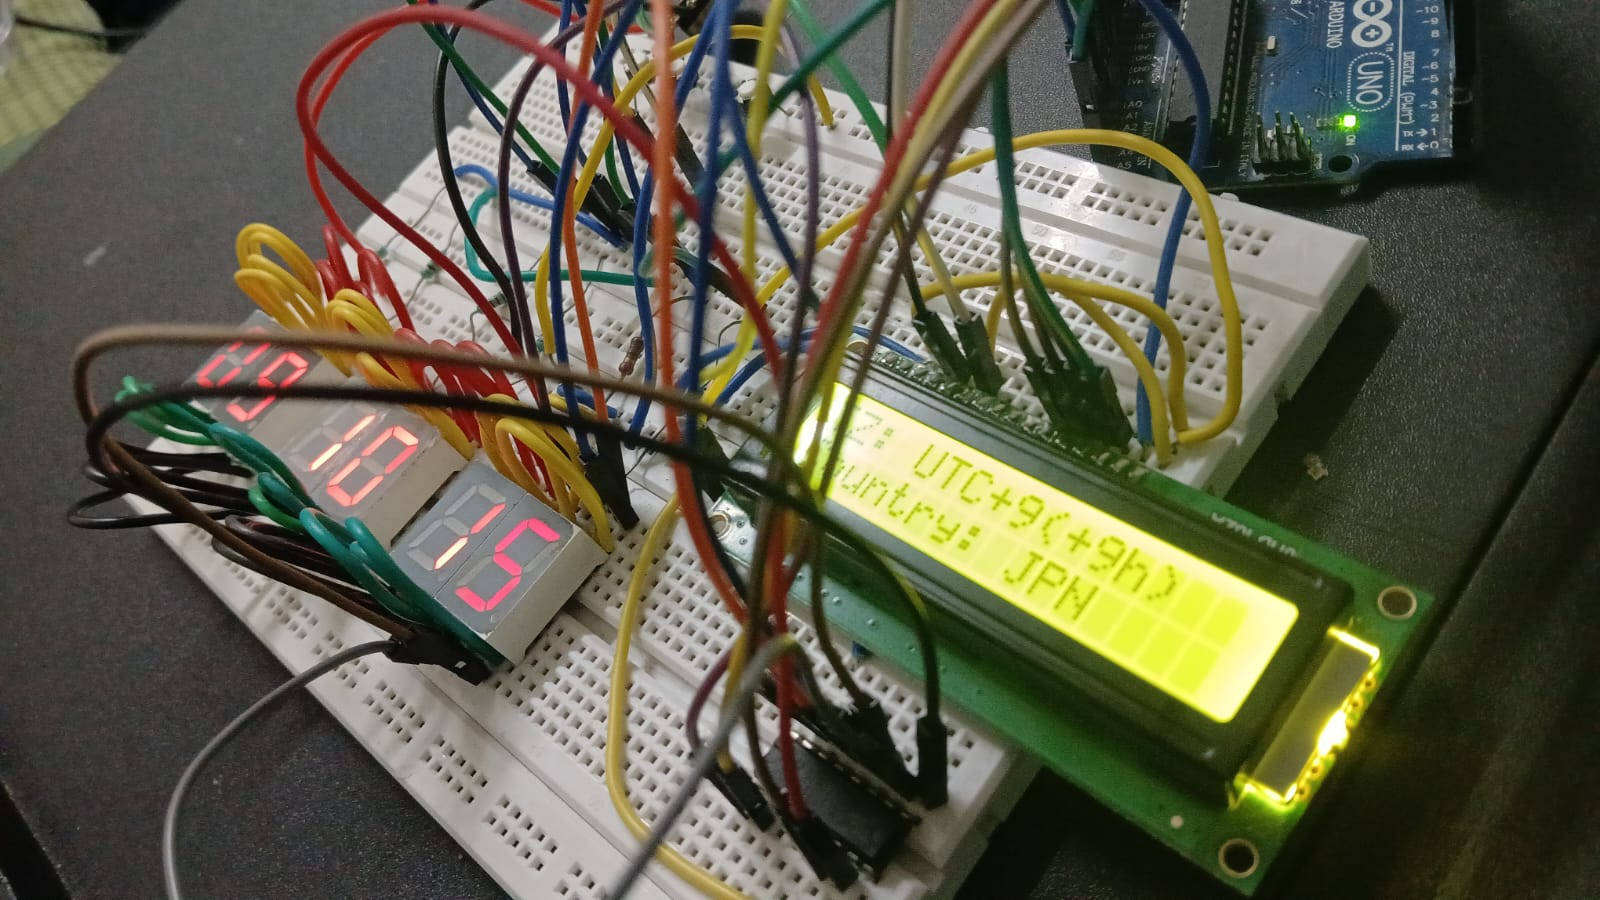
\includegraphics[width=0.8\linewidth]{figs/Clock2.jpeg}
    \caption{Clock}
    \label{fig:enter-label}
\end{figure}

\section{Advatanges of AVR-GCC over other}
\begin{itemize}
    \item Optimized Code for Real-Time Execution
    \item Offers optimized ISR vector mapping for fast execution with low latency.
    \item Supports direct manipulation of AVR hardware registers, which results in faster response times than higher-level abstraction layers.
    \item Direct register-level programming (e.g., TCCR0A, OCR0A, TIMSK1) is completely compatible with different AVR devices.
\item Precise Handling of Button Debouncing
    \item Highly optimized AVR-Libc functions, which minimize RAM and Flash usage.
    \item Efficient register usage, ensuring that conversions and LCD updates do not introduce significant computational delays.
    \item Robust Bitwise Operations for Fast Multiplexing
    \begin{itemize}
    \item Streamlined inline assembly translation with lower instruction cycles for enhanced performance.
    \item Low RAM overhead due to bitwise operations' lack of memory allocations.
    \end{itemize}
\end{itemize}
\section{Code}
{Code for the Digital CLock}
\lstset{
        language = C,
        basicstyle=\ttfamily\tiny,
        keywordstyle=\color{blue},
        stringstyle=\color{green},
        commentstyle=\color{gray},
        tabsize=4
    }
\lstinputlisting{./codes/clock.c}

\section{Precautions}
\subsection{Hardware}
\begin{enumerate}
    \item  Always use ${220}{\ohm}$ resistors in series with the seven-segment display segments to avoid drawing too much current and possibly damaging the Arduino.
    \item  Double-check wiring to avoid short circuits by mistake, which may damage the microcontroller or display.
    \item First of all, cut off the power supply to the Arduino before changing anything in the circuit to avoid any accidental destruction.
\end{enumerate}

\subsection{Software}
\begin{enumerate}
    \item Set the delay of the multiplexing loop such that it will not flicker or display illegible digits. A 1.5-5ms delay per digit is good.
    \item Double-check before uploading code that the appropriate pins are connected to the segments and common anodes of the display.
\end{enumerate}
\end{document}